\documentclass[a4paper,12pt,titlepage]{article}
\usepackage[utf8]{inputenc}
\usepackage{graphicx} % Required for inserting images
\usepackage[spanish,es-tabla]{babel}
\usepackage[none]{hyphenat}
\usepackage[justification=centering]{caption}
\usepackage{subcaption}
\usepackage{amssymb, amsmath}
\usepackage{gensymb}
\usepackage{fancyhdr}
\usepackage{wrapfig}


\title{Oscilador amortiguado y forzado}
\author{Gonzalo Bastos González}

\usepackage[a4paper]{geometry}
\geometry{top=2cm, bottom=2.0cm,left=2cm, right=2cm}

\begin{document}

\begin{center}
    \textbf{\Large Oscilador amortiguado forzado}
\end{center}

\begin{center}
    \textbf{Gonzalo Bastos González}
\end{center}

\section{Oscilador amortiguado}

Partiremos de un péndulo de Pohl descrito por la ecuación:

\begin{equation}
    \theta(t) = \theta_0 e^{-\gamma t} \cos (\omega_1t)
    \label{thetaT}
\end{equation}

Donde $\theta_0$ es la amplitud inicial del péndulo, $\omega_1$ la frecuencia y $\gamma$ es el coeficiente de amortiguamiento. Los máximos de amplitud vendrán dados por la ecuación:

\begin{equation}
    \theta_{max}(t) = \theta_0 e^{-\gamma t}
    \label{A max}
\end{equation}

\subsection{Obtención experimental de $\omega_1$ y $\gamma$}

El coeficiente $\gamma$ de amortiguamiento es característico del movimiento de un oscilador armónico sometido a una fuerza de rozamiento del tipo $F=-kx$, siendo $\gamma$ directamente proporcional a la fuerza. En nuestro caso el amortiguamiento está causado principalmente por el electroimán, que crea las denominadas como corrientes de Foucault al suministrarle una intensidad de corriente $I$. Para el estudio de nuestro oscilador vamos a obtener el valor de $\omega_1$ de forma directa a partir del tiempo de $n$ oscilaciones y vamos a calcular $\gamma$ mediante un ajuste a la ecuación (\ref{A max}).

\par Antes de empezar a exponer las medidas tomadas es importante explicar brevemente la escala de medida del péndulo de Pohl. El péndulo cuenta con una serie de marcas que van desde $-20$ a $20$ a intervalos de $0,2$ y representan el ángulo $\theta$ de oscilación, pero las unidades de este ángulo son arbitrarias.

\par Otro aspecto importante a tratar antes de exponer las medidas son las incertidumbres empleadas. Para las frecuencias $\omega_1$ la incertidumbre vendrá de la medida del tiempo de $n$ oscilaciones a partir de propagación, tomaremos como incertidumbre de los tiempos medidos el doble del tiempo medio de reacción a un estímulo visual, ya que consideramos que el error aumentaba al tener que coordinarnos entre los compañeros para poner en marcha el péndulo, por tanto $s(t)=0,5\; s$. Para los valores de ángulo del péndulo la incertidumbre será la longitud del intervalo de medida más pequeño, por lo que $s(\theta)=0,2$. Por último, la incertidumbre de la intensidad viene dada por el polímetro empleado para medirla, $s(I)=0,01\;A$.

\par Mediremos los valores de $\omega_1$ para diferentes valores de intensidad, comenzando con $I_1=0$. Medimos el tiempo para $n=30$ oscilaciones en 4 ocasiones y calculamos la media. A partir de ahí calculamos $\omega_1$ y su incertidumbre:

\begin{equation}
    \begin{gathered}
        \omega_{1} = \frac{2\pi n}{t} \Rightarrow s(\omega_1) = \frac{s(t)}{t^2}= 0,00016 \;s^{-1}\\
        \omega_{11} = 3,330 \pm 0,030 \;s^{-1}
    \end{gathered}
\end{equation}

Para calcular $\gamma$ (que depende solo del rozamiento del péndulo en este caso) vamos a ajustar los valores de amplitud máxima medidos en función del tiempo, tomando medidas cada dos períodos ($T=2\pi/\omega_1=1,887 \;s$). El ajuste será a una función del tipo $\theta_{max}=ae^{-bt}$, donde $a$ es la amplitud inicial y $b=\gamma$. Obtuvimos los siguientes valores:

\begin{equation}
    \begin{gathered}
        a = \theta_0 = 17,998\pm 0,075 \; u \\
        b = \gamma_1 = 0,006642 \pm  0.00022 \; s^{-1}
    \end{gathered}
\end{equation}

Para $I_2=0,3\;A$ tomamos 5 medidas con $n=10$ oscilaciones para calcular $\omega_{12}$. Para medir la amplitud máxima en función del tiempo medimos estos máximos para cada período:

\begin{equation}
    \omega_{12} = \frac{2n\pi}{t} = 3,361 \pm 0,090\; s^{-1}
\end{equation}

Para calcular $\gamma$ vamos a ajustar los datos a una curva igual que la anterior, del tipo $\theta_{max}=ae^{-bt}$ con $a\equiv \theta_0$ y $b\equiv \gamma$. Obtuvimos que:

\begin{equation}
    \begin{gathered}
        a = \theta_0 = 18,04\pm 0,10 \; u \\
        b = \gamma_2 = 0,10221 \pm 0,00092 \; s^{-1}
    \end{gathered}
\end{equation}

\begin{figure}[h!]
    \centering
    \begin{subfigure}{0.45\textwidth}
        \centering
        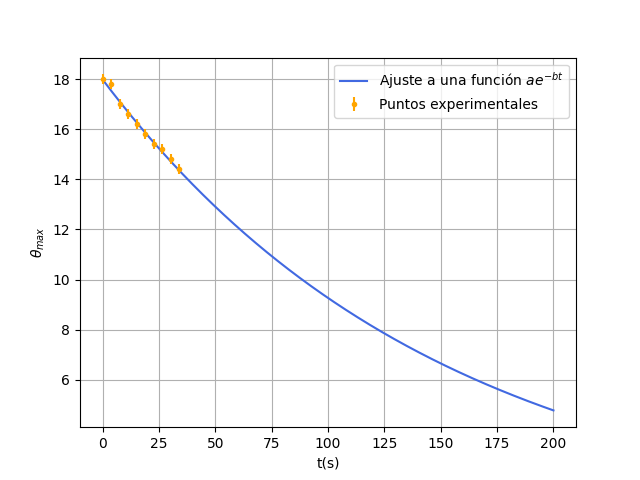
\includegraphics[width=1.1\linewidth]{Images/I0ajuste.png}
        \subcaption{Medidas de $\theta_{max}$ y ajuste para $I=0\;A$}
    \end{subfigure}
    \begin{subfigure}{0.45\textwidth}
        \centering
        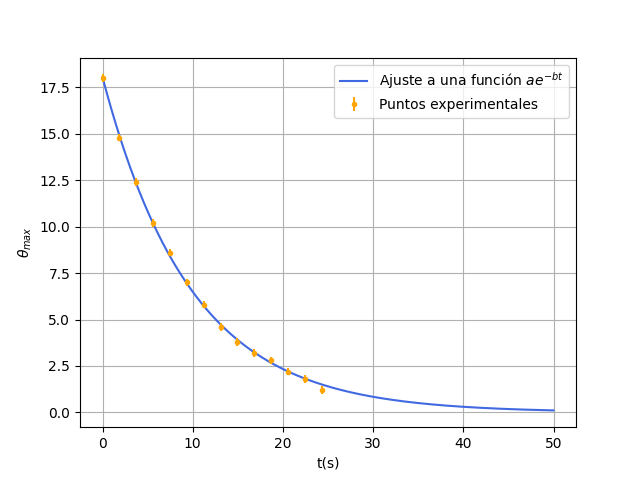
\includegraphics[width=1.1\linewidth]{Images/I3ajuste.png}
        \subcaption{Medidas de $\theta_{max}$ y ajuste para $I=0,3\;A$}
    \end{subfigure}
    \caption{Curvas de amplitudes máximas para $I=0$ y $I=0,3$}
\end{figure}

Para $I_3=0,6\;A$ y todos los siguientes valores de intensidad medimos la amplitud máxima cada semiperíodo. Esto nos va a permitir realizar otros dos ajustes, ya que medimos los máximos y los mínimos ($\theta_{min}=-\theta_0e^{-\omega_1t}$) de la amplitud. Gracias a esto podemos ajustar también a la función cuasiperiódica que describe el movimiento del oscilador, la Ec.\ref{thetaT}. Para medir $\omega_1$ en este caso realizamos 5 medidas con $n=7$ oscilaciones.

\begin{equation}
    \omega_{13} = \frac{2n\pi}{t} = 3,50 \pm 0,14\; s^{-1}
\end{equation}

Para medir la amplitud en función de $t$ tomamos como inicio el lado derecho del péndulo, por lo que $\theta_0>0$ siempre y se corresponderá con $a_{max}$. Obtendremos también la curva para los mínimos y $\theta(t)$:

\begin{equation}
    \begin{gathered}
        a_{max} = \theta_0 = 17,44 \pm 0,38 \quad a_{min} = -\theta_0 = -18,06 \pm 0,38\\
        b_{max} = \gamma =0,376\pm 0,011 \quad b_{min} = \gamma = 0,3812 \pm 0,0083
    \end{gathered}
\end{equation}

Para obtener una expresión para $\theta(t)$ ajustaremos los datos a una curva del tipo \newline $\theta = \theta_0 e^{-bt}\cos(ct+d)$, siendo ${b,c,d}$ los parámetros a determinar.

\begin{equation}
    \begin{gathered}
        b = \gamma = 0,353\pm 0,018 \;s^{-1}\\
        c = \omega_1 = 3,584\pm 0,021 \; s^{-1}\\
        d = \varphi_0 = 0,147 \pm 0,069 
    \end{gathered}
\end{equation}

\begin{figure}[h!]
    \centering
    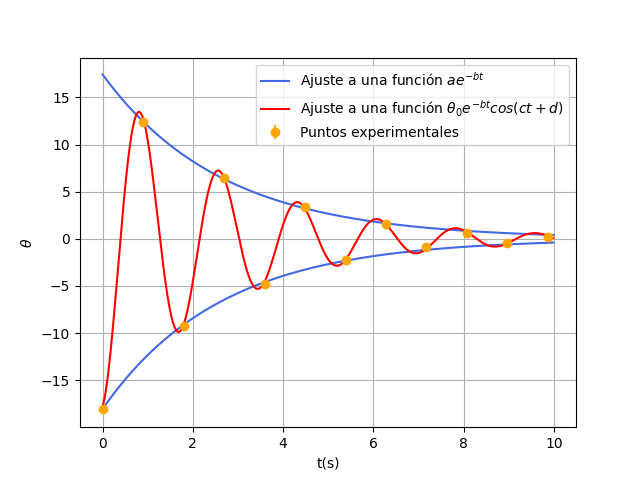
\includegraphics[width=0.65\linewidth]{Images/I6ajuste.png}
    \caption{Medidas de $\theta_{max}$ y ajustes para $I=0,6\;A$}
\end{figure}

\newpage

Para los últimos dos valores de intensidad, $I_4=0,9\,A$ y $I_5=1,1\;A$, el procedimiento es análogo. Para $I_4=0,9\;A$ los resultados obtenidos fueron:

\begin{equation}
    \begin{gathered}
        \omega_{14} =  3.35 \pm 0.22 \; s^{-1} \\
        a_{max} = \theta_0 = 19.80 \pm 0,71 \quad a_{min} = -\theta_0 = -18,02 \pm 0,68\\
        b_{max} = \gamma =0,707\pm 0,022 \quad b_{min} = \gamma = 0,681 \pm 0,022
    \end{gathered}
\end{equation}

Los coeficientes de $\theta(t)$ son:

\begin{equation}
    \begin{gathered}
        b = \gamma = 0,602\pm 0,041 \;s^{-1}\\
        c = \omega_1 = 3,126\pm 0,031 \; s^{-1}\\
        d = \varphi_0 = 0,04 \pm 0,22 
    \end{gathered}
\end{equation}

Para $I_5=1,1\;A$ obtuvimos que:

\begin{equation}
    \begin{gathered}
        \omega_{15} = 3,371 \pm 0,30 \; s^{-1} \\
        a_{max} = \theta_0 = 19.39 \pm 0,85 \quad a_{min} = -\theta_0 = -18,00 \pm 0,058\\
        b_{max} = \gamma =0,8480\pm 0,0082 \quad b_{min} = \gamma = 0,8112 \pm 0,0072
    \end{gathered}
\end{equation}

Los coeficientes de $\theta(t)$ son:

\begin{equation}
    \begin{gathered}
        b = \gamma = 0,764\pm 0,041 \;s^{-1}\\
        c = \omega_1 = 3,177\pm 0,034 \; s^{-1}\\
        d = \varphi_0 = 0,02 \pm 0,23 
    \end{gathered}
\end{equation}

\begin{figure}[h!]
    \centering
    \begin{subfigure}{0.45\textwidth}
        \centering
        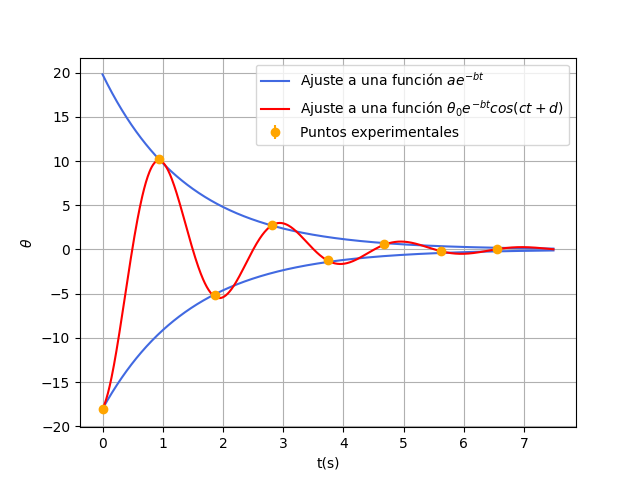
\includegraphics[width=1.05\linewidth]{Images/I9ajuste.png}
        \subcaption{Amplitudes máximas y $\theta(t)$ para $I_4=0,9\;A$}
    \end{subfigure}
    \begin{subfigure}{0.45\textwidth}
        \centering
        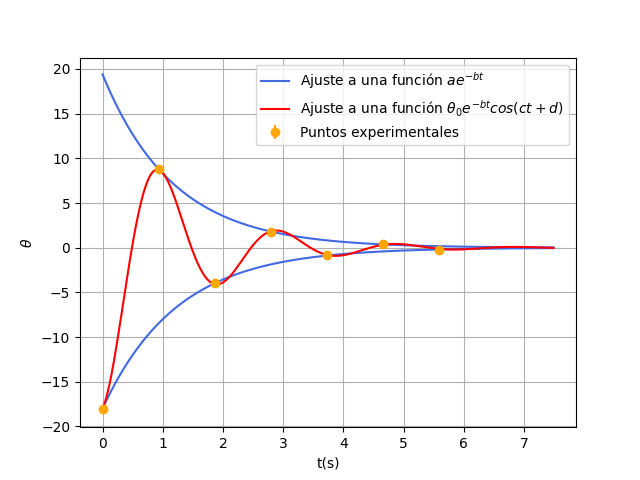
\includegraphics[width=1.05\linewidth]{Images/I11ajuste.png}
        \subcaption{Amplitudes máximas y $\theta(t)$ para $I_4=1,1\;A$}
    \end{subfigure}
    \caption{Ajustes no lineales para $I=,9$ y $I=1,1$}
\end{figure}

\newpage

\subsection{Amortiguamiento crítico y comparación entre $\gamma$ y $\omega_1$}

Una vez obtenidos los valores de $\gamma$ y $\omega_1$ podemos comprobar la veracidad de la ecuación $\omega_1^2 = \omega_0^2-\gamma^2$. Para ello tomaremos $\omega_0\simeq\omega_{11}(I=0\;A)$. Siguiendo esta relación podemos obtener el valor del amortiguamiento crítico, aquel que anula el término $\omega_1$ ($\omega_0=\gamma_c$). El valor $\gamma_c$ se alcanza a una determinada intensidad que interpolaremos ajustando la relación $\gamma(I)$ a una función cuadrática ($\gamma(I)=aI^2+bI+c$). En las siguientes gráficas podemos ver más claros los cálculos hechos.

\begin{figure}[h!]
    \centering
    \begin{subfigure}{0.49\textwidth}
        \centering
        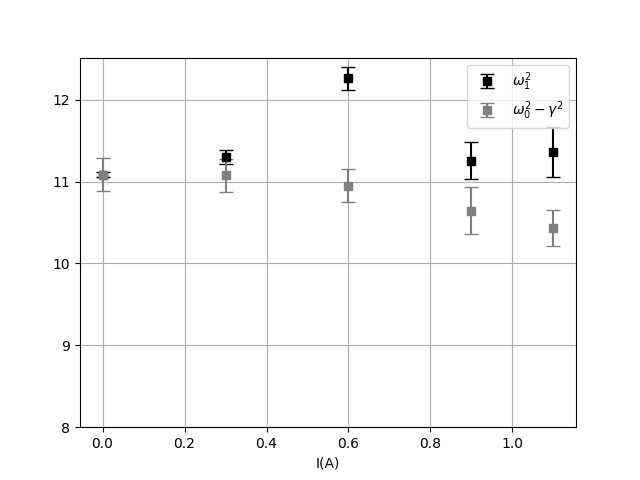
\includegraphics[width=0.95\linewidth]{Images/omega_cuadrado.png}
        \subcaption{Comparación de los valores de $\omega_1^2$ y $\omega_0^2-\gamma^2$}
    \end{subfigure}
    \begin{subfigure}{0.49\textwidth}
        \centering
        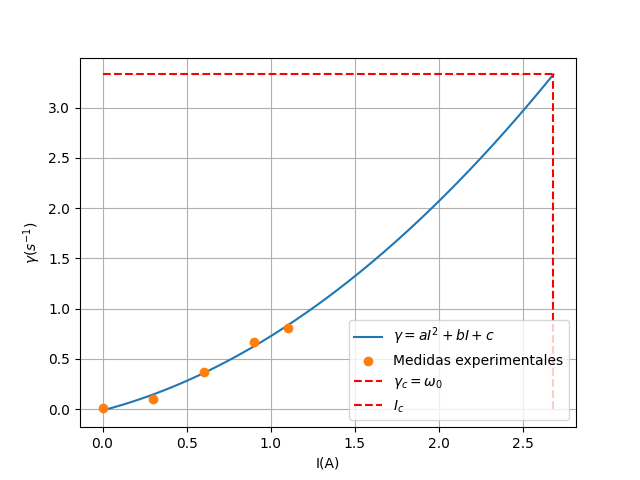
\includegraphics[width=0.95\linewidth]{Images/gammaVSi.png}
        \subcaption{$\gamma(I)=aI^2+bI+c$ y interpolación de la $I_c$}
    \end{subfigure}
    \caption{Estudio del punto de amortiguamiento crítico}
\end{figure}

Como podemos ver en la primera gráfica la relación $\omega_1^2=\omega_0^2-\gamma^2$ no queda del todo clara con las medidas realizadas, los valores de $\omega_1$ medidos no decaen como era de esperar. Esto se puede explicar porque para valores más altos de intensidad medimos el tiempo para de un número pequeño de oscilaciones y el error humano a la hora de medir es en proporción mucho mayor. Por otro lado, después del ajuste cuadrático de $\gamma(I)$ la intensidad crítica, $I_c$, que hace que $\gamma_c=\omega_0$ es:

\begin{equation}
    I_c=2,680 \pm 0,015 \; A
\end{equation}

Este valor se aleja del medido en el laboratorio, $I_c=1,85\pm 0,01 \;A$

\newpage

\section{Oscilador forzado}

En esta parte de la práctica aplicaremos una fuerza periódica al péndulo procedente de un motor. La amplitud del péndulo depende de la frecuencia del motor, $\omega$, de la siguiente forma:

\begin{equation}
    A(\omega) = \frac{F_0/J}{\sqrt{(\omega^2-\omega_0^2)^2+4\gamma^2\omega^2}}
    \label{aw}
\end{equation}

Donde $F_0$ es la fuerza máxima, $J$ el momento de inercia, $\omega$ la frecuencia de la fuerza externa y $\omega_0$ es la frecuencia natural del oscilador. La amplitud tiene un pico cuando $\omega$ se acerca a la denominada frecuencia de resonancia ($\omega_R$) que sigue la siguiente relación que verificaremos:

\begin{equation}
    \omega_R = \sqrt{\omega_0^2-2\gamma^2}
    \label{omegaR}
\end{equation}

Para comprobar este comportamiento medimos las amplitudes máximas para diferentes frecuencias tomando dos intensidades distintas, que provocaban diferentes valores de rozamiento, $I_1=0,3 \;A$ y $I_2=0,6\; A$. Para medir las amplitudes tomamos el valor medio entre el valor máximo de los dos lados del péndulo.

\begin{figure}[h!]
    \centering
    \begin{subfigure}{0.49\textwidth}
        \centering
        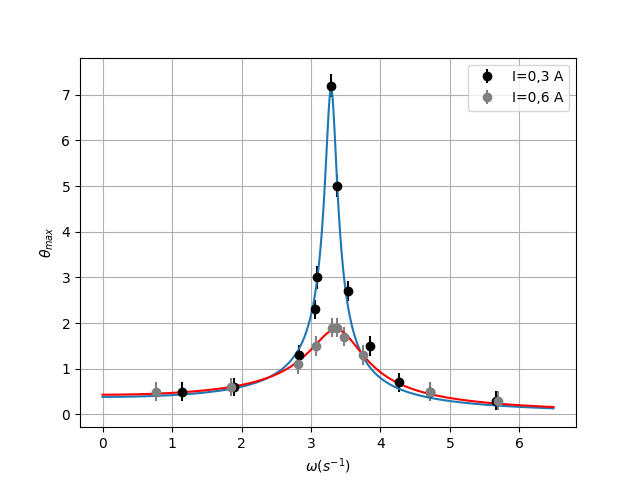
\includegraphics[width=0.95\linewidth]{Images/A(omega).png}
        \subcaption{Medidas experimentales de $A(\omega)$ y ajuste a la Ec.\ref{aw}}
    \end{subfigure}
    \begin{subfigure}{0.49\textwidth}
        \centering
        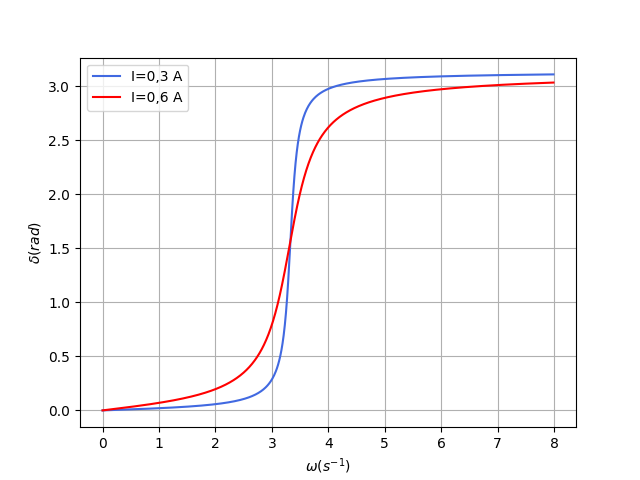
\includegraphics[width=0.95\linewidth]{Images/desfase.png}
        \subcaption{Aproximación de $\delta(\omega)$ para los dos casos estudiados}
    \end{subfigure}
    \caption{Estudio de la resonancia de un oscilador forzado}
    \label{forzado}
\end{figure}

A partir de la gráfica podemos ver la influencia de $\gamma$ en la resonancia, siendo mayor a valores de $\gamma$ bajos y atenúandose mucho cuando hay mucho rozamiento. Esto se puede cuantificar empleando el factor de calidad de nuestro oscilador, que se define como $Q=\omega_R/\Delta \omega$, siendo $\Delta \omega$ la variación entre las frecuencias cuya amplitud es $A=A_R/\sqrt{2}$.

\begin{equation}
    Q_1 = 16,288 \pm 0,026 \quad Q_2= 4,716 \pm 0,016
\end{equation}

Otro aspecto interesante a estudiar es la simetría de la función (\ref{aw}) a ambos lados de su máximo, lo que implica estudiar los casos límite $\omega \to 0$ y $\omega \to \infty$. En primer lugar para el caso $\omega \to 0$ podemos ver que la amplitud tiende a un valor fijo ($\frac{F_0}{J\omega_0}$), no se va a $0$. La interpretación física de esto es que en ese caso límite no habría oscilación de la fuerza, esta sería constante y desplazaría al oscilador de su posición de equilibrio. Para el otro caso límite $\omega \to \infty$ la amplitud sí que se va a $0$. Este caso límite se puede entender mucho mejor si observamos el desfase ($\delta$) que hay entre la fuerza externa y el oscilador. En el laboratorio hicimos un estudio cualitativo de esto, viendo que:

\newpage

\begin{itemize}
    \item En el caso $\omega \to 0 \Rightarrow \delta \to 0$, las oscilaciones están en fase.
    \item En el caso $\omega \to \omega_R \Rightarrow \delta \to \pi/2$, hay medio período de diferencia entre las oscilaciones.
    \item En el caso $\omega \to \infty \Rightarrow \delta \to \pi$, las oscilaciones están en oposición de fase.
\end{itemize}

Por tanto, podemos concluír que la función no es simétrica, pese a que en entornos próximos al máximo si que presenta una alta simetría. Este comportamiento se ve más claro en la Fig.\ref{forzado}, que representa el desfase, $\delta$, en función de $\omega$ a partir de la relación:

\begin{equation}
    \delta = \arctan\left(\frac{2\gamma \omega}{\omega_0^2-\omega^2}\right)
\end{equation}

Los valores obtenidos a partir del ajuste para los coeficientes de la Ec.\ref{aw} fueron:

\begin{equation}
    \begin{gathered}
        (F_0/J)_{(1)} = 4,15 \pm 0,21 \;s^{-1} \quad \omega_{0(1)} = 3,2920 \pm 0,0070 s^{-1} \quad \gamma_{(1)} = 0,0884 \pm 0,0060 \;s^{-1} \\
        (F_0/J)_{(2)} = 5,01 \pm 0,24 \;s^{-1} \quad \omega_{0(2)} = 3,407 \pm 0,020 s^{-1} \quad \gamma_{(2)} = 0,397 \pm 0,022 \;s^{-1}
    \end{gathered}
\end{equation}

A partir de nuestro ajuste interpolamos el valor de $\omega_R$ para las dos intensidades, que se corresponde con el valor de $\omega$ que hace máxima la función. No tiene incertidumbre porque no se trata de un cálculo sino de una interpolación realizada con Python. 

\begin{equation}
    \omega_{R1}(I=0,3\;A) = 3,2897 \;s^{-1} \quad \omega_{R2}(I=0,6\;A)= 3,3605 \; s^{-1}
\end{equation}

Con estos datos podemos verficar la relación (\ref{omegaR}), obteniendo resultados bastante satisfactorios. Pese a que no entran dentro del rango de incertidumbre, los valores de $\omega_R^2$ se corresponden bastante con el valor que deberían tener según los valores de $\gamma$ y $\omega_0$ medidos anteriormente. En la siguiente tabla podemos ver también la comparación entre los valores de $\gamma$ obtenidos del ajuste ($\gamma_I$) y los obtenidos en los apartados anteriores ($\gamma_E$). Para $I=0,6\;A$ tomamos como $\gamma$ la media de el valor obtenido para los máximos y para los mínimos de amplitud.

\begin{table}[h!]
    \centering
    \begin{tabular}{c|c|c|c|c|}
    \cline{2-5}
        & $\omega_R^2\;(s^{-2})$ & $\omega_0^2-2\gamma^2\;(s^{-2})$ & $\gamma_I(s^{-1})$ & $\gamma_E(s^{-1})$\\ \hline
    \multicolumn{1}{|c|}{$I=0,3\; A$}  & $10,8221$   &  $11,0652 \pm 0,0011$ & $0,0884\pm0,0060$ & $0,10221 \pm 0,00092$\\ \hline
    \multicolumn{1}{|c|}{$I=0,6\;A$} & $11,293$ & $10,837 \pm 0,016$ & $0,397\pm 0,022$ &  $0,3786 \pm 0,047$ \\ \hline
    \end{tabular}
    \caption{Verificación de la relación $\omega_R^2=\omega_0^2-2\gamma^2$ y de los valores de $\gamma$ obtenidos}
    \label{tab:my-table}
    \end{table}

\section{Conclusión}

Nuestra práctica se basa en el estudio de un movimiento oscilatorio que se ve sometido a una fuerza de rozamiento y una fuerza externa oscilante.

\par Cuando solo aplicamos el rozamiento pudimos obtener con éxito la función sinusoidal que describe el movimiento y la función a la que se ajustan los valores máximos de amplitud. Observamos también el fenómeno del amortiguamiento crítico, en el que pudimos ver una clara diferencia entre la $I_c$ medida ($1,85\;A$) y la obtenida a partir de la relación $\gamma(I) (2,68 \;A)$, que supusimos cuadrática.
\par Por otra parte, cuando aplicamos una fuerza externa oscilante nos centramos en estudiar el fenómeno de la resonancia, buscando la frecuencia que maximizaba la amplitud ($\omega_R$). Pudimos observar también la relación entre esta amplificación y el amortiguamiento, en cuanto este subía la resonancia se volvía imperceptible.


\end{document}